\section{MeshConvert}
\label{s:utilities:meshconvert}

MeshConvert is a utility bundled with Nektar++ which primarily allows foreign
mesh file formats to be converted into the XML file format used by the solvers
and other utilities. However, there is also some limited support for other
output formats - consult the MeshConvert reference page for more information on
which formats are supported.

We will run through a basic example to show how a mesh can be
converted from the widely-used mesh-generator Gmsh to the XML file format.


\subsection{Exporting a mesh from Gmsh}

To demonstrate how MeshConvert works, we will define a simple channel-like 3D
geometry.
First, we must define the Gmsh geometry to be used. The Gmsh definition is given
below, and is visualised on the right.

\begin{lstlisting}[style=XmlStyle]
Point(1) = {-1, 0, 0, 1.0};
Point(2) = {-0.3, 0, 0, 1.0};
Line(3) = {1, 2};
s[] = Extrude {0, 0, 7} {
  Line{3}; Layers{5}; Recombine;
};
v[] = Extrude {{0, 0, 1}, {0, 0, 0}, Pi} {
  Surface{s[1]}; Layers{10}; Recombine;
};
\end{lstlisting}

Whilst a full tutorial on Gmsh is far beyond the scope of this document, note
the use of the Recombine argument. This allows us to generate a structured
hexahedral mesh; remove the first Recombine to generate a prismatic mesh and
both to generate a tetrahedral mesh. Increasing the `Layers' numbers refines the
mesh in the radial and azimuthal direction respectively.

\subsection{Defining physical surfaces and volumes}

In order for us to use the mesh, we need to define the physical surfaces which correspond to the inflow, outflow and walls so that we can set appropriate boundary conditions. The numbering resulting from the extrusions in this case is not straightforward. In the graphical interface, select Geometry > Physical Groups > Add > Surface, and then hover over each of the surfaces which are shown by the dashed gray lines. The numbering will be revealed in the toolbar underneath the geometry as a ruled surface. In this case:
\begin{enumerate}
\item Walls: surfaces 7, 8, 28, 29.
\item Inflow: surface 16.
\item Outflow: surface 24.
\end{enumerate}

We also need to define the physical volumes, which can be done in a similar fashion. For this example, there is only one volume having ID 1. Adding these groups to the end of the `.geo' file is very straightforward:

\begin{lstlisting}[style=XmlStyle] 
Physical Volume(0) = {1}; 
Physical Surface(1)= {7,8,28,29}; 
Physical Surface(2) = {16}; 
Physical Surface(3) = {24};
\end{lstlisting}
Either choose the option \inlsh{File->Save Mesh} or, assuming this is saved in
a file named `test.geo', run the command 
\begin{lstlisting}[style=BashInputStyle]
gmsh -3 test.geo
\end{lstlisting}
which will produce the resulting MSH file `test.msh'. One can generate a
high-order mesh by specifying the order on the command line, for example
\begin{lstlisting}[style=BashInputStyle] 
gmsh -3 -order 6 test.geo
\end{lstlisting}
will generate a sixth-order mesh. Note that you will need to use a current
version of Gmsh in order to do this, most likely from subversion.


\subsection{Converting the MSH to Nektar++ format}
Assuming that you have compiled Nektar++ according to the compilation instructions, run the command
\begin{lstlisting}[style=BashInputStyle]
MeshConvert test.msh test.xml
\end{lstlisting}
to generate the XML file. 

\begin{notebox}
This file contains only the geometry definition (and a default
\inltt{EXPANSIONS} definition). In order to use this mesh, a \inltt{CONDITIONS}
section must be supplied detailing the solver and parameters to use.
\end{notebox}

To validate the mesh visually, we can use a utility such as Paraview or ?VisIt. To do this, run the command
\begin{lstlisting}[style=BashInputStyle]
XmlToVtk test.xml
\end{lstlisting}
which generates an unstructured VTK file test.vtu


\subsection{MeshConvert modules}
 %------------------------------------------------------------
\subsubsection{Detecting elements with negative Jocabians}
To detect elements with negative Jacobians use :
\begin{lstlisting}[style=BashInputStyle]
MeshConvert -m jac Mesh.xml
\end{lstlisting}
and to extract the elements (in order to visualize them for example) use :
\begin{lstlisting}[style=BashInputStyle]
MeshConvert -m jac:extract Mesh.xml MeshWithNegativeElements.xml
\end{lstlisting}
 %------------------------------------------------------------
\subsubsection{Periodic boundary conditions}
Gmsh and Nektar++ use different edge ordering and surface orientation. To use periodic boundary conditions the faces must be aligned properly. To make sure faces (or edges for a 2D mesh) are aligned correctly use the following command :
\begin{lstlisting}[style=BashInputStyle]
MeshConvert -m peralign:surf1=11:surf2=12:dir=y \
    -m peralign:surf1=13:surf2=14:dir=z Mesh.xml Mesh_aligned.xml
\end{lstlisting}
where the surfaces "11" and "12" will be aligned normal to "y" and the surfaces "13" and "14" will be aligned normal to "z". Mind the double use of the "-m"! Mesh.xml is the initial mesh by Gmsh and \verb+Mesh_aligned.xml+ is the new mesh output by this command with aligned surfaces (or edges).
 %------------------------------------------------------------
\subsubsection{Spherigon Patches}
To use spherigon patches on two contiguous surfaces "11" and "12" use the following command :
\begin{lstlisting}[style=BashInputStyle]
MeshConvert -m spherigon:surf=11,12 \
    MeshWithStraighEdges.xml MeshWithSpherigons.xml
\end{lstlisting}
If the two surfaces "11" and "12" are not contiguous use :
\begin{lstlisting}[style=BashInputStyle]
MeshConvert -m spherigon:surf=11 -m spherigon:surf=12 \
    MeshWithStraighEdges.xml MeshWithSpherigons.xml
\end{lstlisting}
If you have a high-resolution mesh of the surfaces "11" and "12" in ".ply " format it can be used to improve the normal definition of the spherigons. Run :
\begin{lstlisting}[style=BashInputStyle]
MeshConvert -m spherigon:surf=11,12:usenormalfile=Surf_11-12_Mesh.ply \
    MeshWithStraighEdges.xml MeshWithSpherigons.xml 
\end{lstlisting}
This can be useful, for example, when meshing the Leading edge of an airfoil. Starting from a "linear" mesh (Fig.1) the spherigon patches curve the surface elements producing leading edge closer to the underlying geometry :
\begin{figure}[!htbp]
\begin{center}
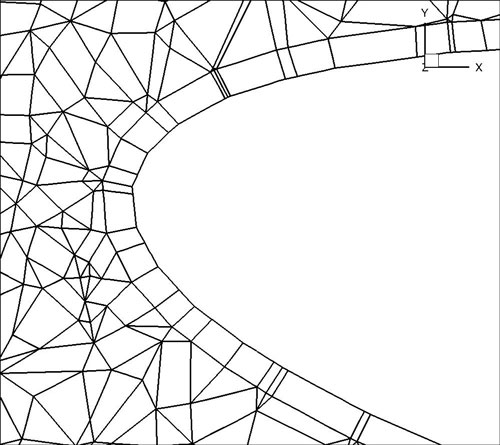
\includegraphics[width = 0.47 \textwidth]{Figures/noSphnoBL.jpg}
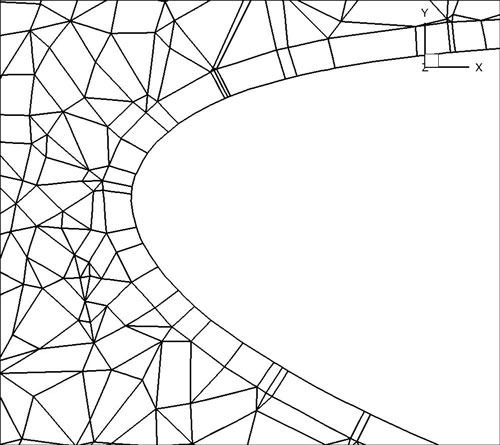
\includegraphics[width = 0.47 \textwidth]{Figures/SphnoBL.jpg}
\caption{(a) LE without Spherigons, (b) LE with Spherigons}
\label{fig:}
\end{center}
\end{figure}
 %------------------------------------------------------------
\subsubsection{Prism splitting}
To split a prism boundary layer on surface "11" into 3 layers with a growth rate of 2 and 7 integration points per element use the following command :
\begin{lstlisting}[style=BashInputStyle]
MeshConvert -m bl:surf=11:layers=3:r=2:nq=7 MeshWithOnePrismLayer.xml \
        MeshWith3PrismsLayers.xml
\end{lstlisting}
\begin{figure}[!htbp]
\begin{center}
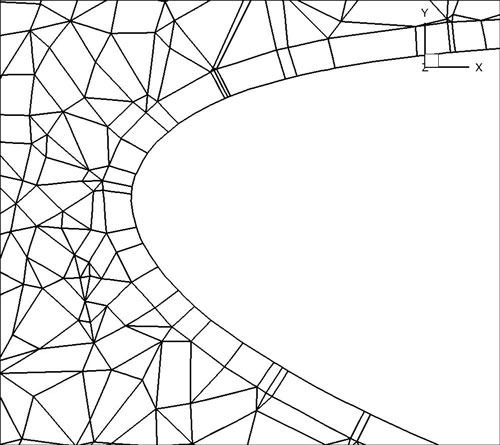
\includegraphics[width = 0.47 \textwidth]{Figures/SphnoBL.jpg}
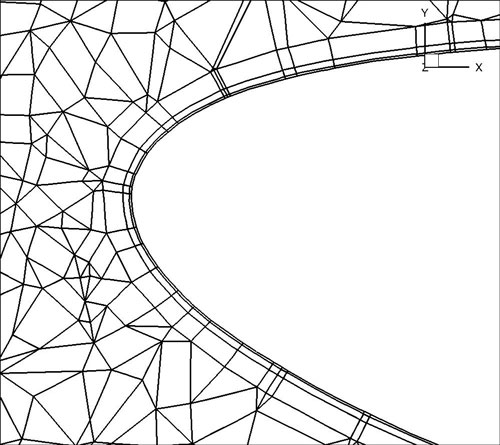
\includegraphics[width = 0.47 \textwidth]{Figures/SphBL.jpg}
\caption{(a) LE with Spherigons but only one prism layer for resolving the boundary layer, (b)  LE with Spherigons with 3 growing layers of prisms for better resolving the boundary layer.}
\label{fig:}
\end{center}
\end{figure}

\subsubsection{High-order cylinder generation}
Generating accurate high-order curved geometries in Gmsh is quite challenging.
This module processes an existing linear cylindrical mesh, with axis aligned
with the z-coordinate axis, to generate accurate high-order curvature
information along the edges.
\begin{lstlisting}[style=BashInputStyle]
MeshConvert -m cyl:surf=2:r=1.0:N=5 LinearCylinder.xml HighOrderCylinder.xml
\end{lstlisting}
The module parameters are:
\begin{itemize}
    \item \inlsh{surf}: Surface on which to apply curvature. This should be the
        outer surface of the cylinder.
    \item \inlsh{r}: Radius of the cylinder.
    \item \inlsh{N}: Number of high-order points along each element edge.
\end{itemize}

\begin{notebox}
    The module could also be used to apply curvature along the interior of a
    hollow cylinder. However, there are no checks to ensure the resulting
    elements are not self-intersecting.
\end{notebox}
